\begin{frame}{Деревья}
\begin{figure}[ht]
\begin{subfigure}{.49\textwidth}
Хранят элементы по-разному
\begin{itemize}
\item Только в узлах
\item Только в листьях
\item И там, и там
\end{itemize}
\vspace{1em}
По форме бывают разные
\begin{itemize}
\item Бинарные
\item $n$-арные
\item другие
\end{itemize}
\end{subfigure}
\begin{subfigure}{.49\textwidth}
\includegraphics{tikzpics/fig.2.8.before.pdf}\par
\end{subfigure}
\end{figure}
\end{frame}


\begin{frame}
\begin{minipage}{\textwidth}
\begin{minipage}[t]{.48\textwidth}\vspace{0em}
  \includegraphics{tikzpics/fig.2.8.before.pdf}\par
\end{minipage}
\begin{minipage}[t]{.48\textwidth}\vspace{0em}
  \includegraphics{tikzpics/fig.2.8.after.pdf}\par
\end{minipage}
\end{minipage}
Выполнение \texttt{ys $\equiv$ add("e",xs)}.\\

Для большинства деревьев путь, который надо изменить, содержит лишь небольшую долю узлов в дереве. Громадное
большинство узлов будет находиться в совместно используемых поддеревьях.
\end{frame}

\subsection{Двоичные деревья поиска}

\begin{frame}{Двоичные деревья поиска}
\begin{definition}[Двоичные деревья поиска]
Двоичные деревья, в которых элементы cимметричном
 (symmetric) порядке, то есть, элемент в каждом узле больше любого элемента в левом поддереве
этого узла и меньше любого элемента в правом поддереве. 
\end{definition}
\end{frame}

\begin{frame}{Двоичные деревья поиска: вставка}
Например, пусть двоичное дерево поиска каких-то значений -- это 
\begin{itemize}
\item Либо лист без значений
\item Либо узел, который хранит значение и двое других двоичных деревьев поиска
\end{itemize}
\vspace{1em}

Функция \mlinline{insert: tree*int -> tree} вставки значения $x$ в дерево:
\begin{itemize}
\item Вставка в пустое дерево тривиальна
\item Иначе наше дерево -- это узел из значения $y$ и двух других поддеревьев \mlinline{l} и \mlinline{r}
\begin{itemize}
\item Если $x<y$, то ответ -- это дерево из $y$, \mlinline{insert x l} и \mlinline{r}
\item Если $x>y$, то ответ -- это дерево из $y$, \mlinline{l} и \mlinline{insert x r} 
\item Иначе не нужно добавлять, дерево из $y$, \mlinline{l} и \mlinline{r} -- это ответ
\end{itemize}
\end{itemize}
\vspace{2em}
Функция \mlinline{member: tree*int -> bool} пишется аналогично
\end{frame}

%
%\begin{frame}
%3+2 упражнения на 22й странице
%\end{frame}






\subsection{Красно-чёрные деревья}

\begin{frame}{Красно-чёрные деревья}
Двоичные деревья поиска хорошо ведут себя на случайных или неупорядоченных данных,
однако на упорядоченных данных их производительность резко падает, и
каждая операция может занимать до $O(n)$  времени. \\

 Решение этой
проблемы состоит в том, чтобы каждое дерево поддерживать в
приблизительно сбалансированном состоянии. Тогда каждая операция
выполняется не хуже, чем за время $O(\log n)$. \\

 Одним из наиболее
популярных семейств сбалансированных двоичных деревьев поиска являются
красно-чёрные.
\end{frame}

\begin{frame}[fragile]{}{Красно-чёрные деревья}

\begin{definition}[Красно-чёрные деревья]
Это двоичные деревья поиска особой структуры
\begin{itemize}
\item либо узел, состоящий из цвета, значения и двух поддеревьев
\begin{itemize}
\item где цвет бывает либо красный, либо черный
\end{itemize}
\item либо лист без значений (считается черным)
\end{itemize}
\end{definition}
\vspace{1em}


Мы требуем, чтобы всякое красно-чёрное дерево соблюдало два
инварианта:
\begin{itemize}
  \item \textbf{Инвариант 1.} У красного узла не может быть красного ребёнка.
  \item \textbf{Инвариант 2.} Каждый путь от корня дерева до пустого
  узла содержит одинаковое количество чёрных узлов.
\end{itemize}
Вместе эти два инварианта гарантируют, что самый длинный возможный
путь по красно-чёрному дереву, где красные и чёрные узлы чередуются,
не более чем вдвое длиннее самого короткого, состоящего только из
чёрных узлов.

%\ifanswers
%\begin{exercise}\label{ex:3.8}
%  Докажите, что максимальная глубина узла в красно-чёрном дереве
%  размера $n$ не превышает $2 \lfloor \log (n+1) \rfloor$.
%\end{exercise}
%\fi
\end{frame}


\begin{frame}{Вставка делается нетривиально}
%Например, пусть двоичное дерево поиска каких-то значений -- это 
%\begin{itemize}
%\item Либо лист без значений
%\item Либо узел, который хранит значение и двое других двоичных деревьев поиска
%\end{itemize}
%\vspace{1em}

Функция \mlinline{insert: tree*int -> tree} вставки значения $x$ в дерево реализуется с помощью функции 
\mlinline{balance}:
\begin{itemize}
\item Вставка в пустое дерево тривиальна
\item Иначе вставляем в  дерево, которое состоит из: значения $y$, цвета $c$ и двух других поддеревьев \mlinline{l} и \mlinline{r}
\begin{itemize}
\item Если $x=y$, то возвращаем дерево как есть
\item Если $x<y$, нужно вызвать \mlinline{balance(c, insert x l, y, r)} 
\item Если $x>y$, нужно вызвать \mlinline{balance(c, l, y, insert x r)} 
\end{itemize}
\end{itemize}
\vspace{2em}
Функция \mlinline{balance: color*tree*int*tree -> tree} конструирует узел дерева, переупорядочивая, если нужно
\end{frame}

%\defverbatim[colored]{\balance}{
%\begin{minted}{ocaml}
%let balance = function
%  | B, T (R, T (R, a, x, b), y, c), z, d
%  | B, T (R, a, x, T (R, b, y, c)), z, d
%  | B, a, x, T (R, T (R, b, y, c), z, d)
%  | B, a, x, T (R, b, y, T (R, c, z, d)) ->
%      T (R, T (B, a, x, b), y, T (B, c, z, d))
%  | c, a, x, b -> T (c, a, x, b)
%\end{minted}
%}

%\begin{frame}[fragile]{Балансировка}
%Функция \mlinline{balance} действует подобно
%конструктору \mlinline{T}, но только она переупорядочивает свои
%аргументы, чтобы обеспечить выполнение инвариантов баланса.
%\vspace{1em}
%
%\balance
%\vspace{1em}
%
%Почему выполняется Инвариант 2 будет видно на картинке.
%
%Инвариант 1 будет нарушаться только временно, по мере перебалансирования снизу вверх
%\end{frame}


%\begin{frame}[fragile]{}
%Функция
%\hsinline{balance} обнаруживает и исправляет красно-красные нарушения,
%когда обрабатывает чёрного родителя красного узла с красным
%ребёнком. Такая чёрно-красно-красная цепочка может возникнуть в
%четырёх различных конфигурациях, в зависимости от того, левым или
%правым ребёнком является каждая из красных вершин. Однако в каждом из
%этих случаев решение одно и то же: нужно преобразовать
%чёрно-красно-красный путь в красную вершину с двумя чёрными детьми,
%как показано на рисунке ниже.
%
%После балансировки некоторого поддерева красный корень этого поддерева
%может оказаться ребёнком ещё одного красного узла. Таким образом,
%балансировка продолжается до самого корня дерева. На самом верху
%дерева мы можем получить красную вершину с красным ребёнком, но без
%чёрного родителя. С этим вариантом мы справляемся, всегда перекрашивая корень
%в чёрное.
%
%\end{frame}


\begin{frame}[fragile]{}
\begin{figure}[h]
  \centering
  \documentclass[tikz]{standalone}

\usepackage{tikz}
\usetikzlibrary{positioning,trees,decorations.pathreplacing}

\begin{document}
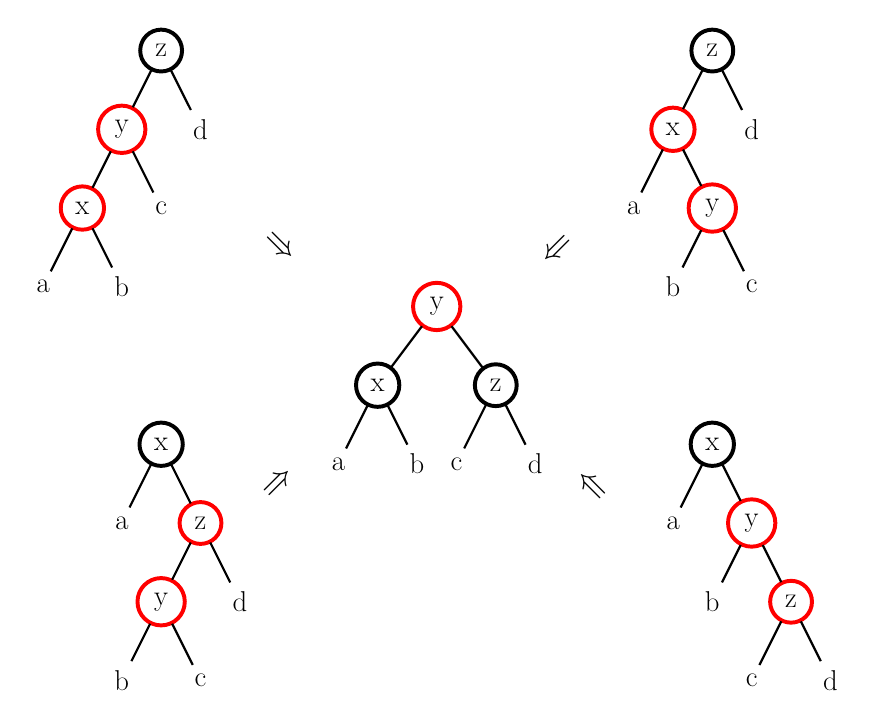
\begin{tikzpicture}[thick,scale=0.5, every node/.style={scale=0.5},level distance=2cm, sibling distance=2cm]
    \tikzstyle{tblack}=[circle, line width=.5mm, draw=black]
    \tikzstyle{tred}=[circle, line width=.5mm, draw=red]
    \def\xstep{7cm}
    \def\ystep{5cm}
    
    \huge
    
    % legend
%    \begin{scope}[xshift=7cm, yshift=7cm]
%        \def\inse{3.5mm}
%     %   \draw (-1, -2.5) rectangle (5, 1);
%        
%        \node[tblack, inner sep=\inse] at (0,0) {};
%        \node[tred, inner sep=\inse] at (0,-1.6) {};
%        \node[right=1pt] at (1,0) { -- черный};
%        \node[right=1pt] at (1,-1.6) { -- красный};
%    \end{scope}
    
    \begin{scope}[yshift=\ystep,xshift=\xstep]
        \node[tblack] {z}
            child { node[tred] {x}
                child { node {a} }
                child { node[tred] {y}
                    child {node {b}}
                    child {node {c}}
                }
            }
            child { node {d} };
    \end{scope}
    
    \begin{scope}[yshift=-\ystep,xshift=\xstep]
        \node[tblack] {x}
            child { node {a} }
            child { node[tred] {y}
                child { node {b} }
                child { node[tred] {z}
                    child {node {c}}
                    child {node {d}}
                }
            };
    \end{scope}
    
    \begin{scope}[xshift=-\xstep,yshift=\ystep]
        \node[tblack] {z}
            child { node[tred] {y}
                child { node[tred] {x}
                    child {node {a}}
                    child {node {b}}
                }
                child { node {c} }
            }
            child { node {d} };
    \end{scope}
    
    \begin{scope}[xshift=-\xstep,yshift=-\ystep]
        \node[tblack] {x}
            child { node {a} }
            child { node[tred] {z}
                child { node[tred] {y}
                    child {node {b}}
                    child {node {c}}
                }
                child { node {d} }
            };
    \end{scope}
    
    \begin{scope}[yshift=-1.5cm]
        \tikzstyle{level 1}=[sibling distance=3cm]
        \tikzstyle{level 2}=[sibling distance=2cm]
        \node[tred] {y}
            child { node[tblack] {x}
                child { node {a} }
                child { node {b} }
            }
            child { node[tblack] {z}
                child { node {c} }
                child { node {d} }
            };
    \end{scope}
    \Huge
    \draw (3cm, 0cm) node[rotate=-135] {$\Rightarrow$};
    \draw (-4cm, -6cm) node[rotate=45] {$\Rightarrow$};
    \draw (-4cm, 0cm) node[rotate=-45] {$\Rightarrow$};
    \draw (4cm, -6cm) node[rotate=135] {$\Rightarrow$};
    
\end{tikzpicture}

\end{document}


\end{figure}
\end{frame}



%\subsection{Расширяющиеся (splay) деревья}



%\begin{frame}[fragile]{}
%%\begin{hint}
%  Даже без дополнительных оптимизаций наша реализация сбалансированных
%  двоичных деревьев поиска~--- одна из самых быстрых среди
%  имеющихся. С оптимизациями вроде описанных в
%  Упражнениях~\ref{ex:2.2} и \ref{ex:3.10} она просто летает!
%%\end{hint}
%\end{frame}


%\begin{frame}{Почему это выглядит короче императивной реализации?}
%\begin{remark}
%  Одна из причин, почему наша реализация выглядит настолько проще, чем
%  типичное описание красно-чёрных деревьев, состоит в том, что мы
%  используем несколько другие преобразования перебалансировки. 
%  \vspace{1em}
%  
%  В императивных реализациях обычно наши четыре проблематичных случая
%  разбиваются на восемь, в зависимости от цвета узла, соседствующего с
%  красной вершиной с красным ребёнком.  Знание цвета этого узла в
%  некоторых случаях позволяет совершить меньше присваиваний, а в
%  некоторых других завершить балансировку раньше. Однако в
%  функциональной среде мы в любом случае копируем все эти вершины, и
%  таким образом, не можем ни сократить число присваиваний, ни
%  прекратить копирование раньше времени, так что для использования
%  более сложных преобразований нет причины.
%\end{remark}
%\end{frame}


\subsection{Префиксные деревья}

\begin{frame}{Префиксные деревья (trie)}
\begin{figure}[ht]
\begin{subfigure}[t]{.33\textwidth}
Желаем хранить последовательности так, чтобы начинающиеся с одного и того же были рядом
\end{subfigure}\hspace{0em}
\begin{subfigure}[t]{.65\textwidth}
\begin{center}
\includegraphics[page=1,scale=1.1]{tikzpics/trie1.pdf}
\end{center}
%Картинка \href{https://tex.stackexchange.com/a/182484/171947}{отсюда}
\end{subfigure}
\end{figure}
\end{frame}

\begin{frame}{Префиксные деревья (trie)}
\begin{figure}[ht]
\begin{subfigure}[t]{.33\textwidth}\vspace{0em}
Можно сжимать ребра, ускоряя доступ к листу, но увеличивая количество ветвей\\%\vspace{1em}

Если сжать их до максимума, то структура начнет напоминать массив\\

%На практике количесво 
\end{subfigure}\hspace{0em}
\begin{subfigure}[t]{.65\textwidth}\vspace{0em}
\begin{center}
\includegraphics[page=2,scale=1]{tikzpics/trie1.pdf}
\end{center}
\end{subfigure}
\end{figure}
\end{frame}


\begin{frame}{Префиксные деревья (trie), где ключи -- числа}
\begin{figure}[ht]
\begin{subfigure}{.39\textwidth}
Конечное отображение (map)
\begin{itemize}
\item $63=11111_2\mapsto$ Bauer 
\item $31=01111_2\mapsto$ Baum 
\item $2=10_2\mapsto$ Hof 
\item $71=100111_2\mapsto$ Huhn
\item $39=010111_2\mapsto$ Hund
\end{itemize}
\end{subfigure}
\begin{subfigure}{.59\textwidth}
\includegraphics[page=3,scale=1.4]{tikzpics/trie1.pdf}
\end{subfigure}
\end{figure}
\vspace{2em}
Важный апгрейд: HAMT (Hash Array Mapped Trie)
\end{frame}
